\documentclass[a4paper]{article}

\usepackage{amsmath}
\usepackage{amssymb}
\usepackage{graphicx}
\usepackage{physics}
%\usepackage[round]{natbib}
%\usepackage{bibtex}
\usepackage{fancyvrb}
\usepackage{hyperref}
\usepackage[linesnumbered,boxed]{algorithm2e}
\usepackage{subfigure}

\numberwithin{equation}{section} % Remove this line for global equation numbering

\title{Stefano's awesome MATH1058 coursework report}
\author{Stefano Coniglio}
\date{\today}

\begin{document}

% This produces the title: to modify contents, change the \title, \author, and
% \date in the preamble
\maketitle

\begin{abstract}
  This document reports on something really interesting, hopefully.
\end{abstract}

\section{Introduction}
\label{sec:intro}

We consider, in this work, a definitely relevant problem which, in formal terms, can be expressed as follows:
%
\begin{quote}
  {\bf Very Interesting Problem (VIP):} Given a quite relevant set of givens $A \in \mathbb{R}^{m \times n}, b \in \mathbb{R}^n, c \in \mathbb{R}^n$, the VIP problem calls for a very, very relevant solution $x \in \mathbb{R}^n$ which satisfies the following very, very, very (!) relevant property:
  \begin{equation}\label{equation:theRelevantOne}
    z = \max_{x \in \mathbb{R}^n_+} \{cx: Ax \leq b\}
  \end{equation}
\end{quote}

Relying on Equation~\eqref{equation:theRelevantOne}, the algorithm computes $x$ proceeding according to the following pseudocode:

\begin{algorithm}[H]\label{alg:theGoodOne}
 \KwData{this text}
 \KwResult{how to write algorithm with \LaTeX2e }
 initialization\;
 \While{not at end of this document}{
  read current\;
  \eIf{understand}{
   go to next section\;
   current section becomes this one\;
   }{
   go back to the beginning of current section\;
  }
 }
 \caption{How to write algorithms.}
\end{algorithm}

The pseudocode reported in Algorithm~\ref{alg:theGoodOne} was taken from~\cite{coniglio}.\footnote{Actually, it was not, but I thought that citing myself was a good idea.}

\section{Solution approach and implementation}

We had a great solution idea, which we implemented in the following beautiful piece of Python code:


\begin{Verbatim}[numbers=left]
def beautiful_function(myUnusedInput, mySecondUnusedInput):
    if do_something_awesome() == True:
        return youWillNeverBugOutOnMe
    else:
        return myVeryUndefinedOutput
\end{Verbatim}


\section{Experimental results and analysis}

We have run a set of experiments on this very costly piece of hardware: {\em xxx}. Our findings are summarized in the quite colorful Figure~\ref{fig:whatANiceFigure}.


\begin{figure}[h]
  \subfigure[]{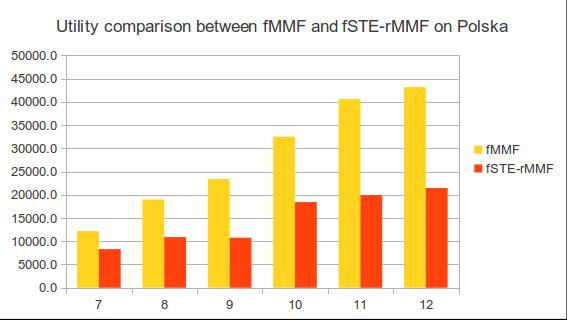
\includegraphics[scale=0.4]{./template_placeholder.png}}
  \subfigure[]{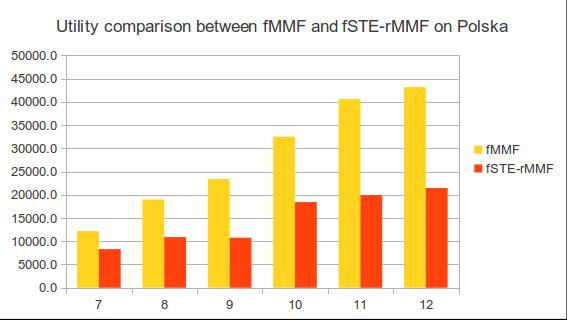
\includegraphics[scale=0.4]{./template_placeholder.png}}
  \caption{One very nice chart entirely unrelated to this coursework (a) and an apparently very similar chart stil unrelated to this coursework (b).}
  \label{fig:whatANiceFigure}
\end{figure}

We should not forget to explain what conclusions the figure allows us to draw, nor why.

Also, including a table may be a good idea. Take a look at Table~\ref{tab:1}:

\begin{table}[htbp]
  \caption{A nice table. Notice that captions preceed tables, whereas they follow figures.}
  \begin{center}
\begin{tabular}{l|lll}
  header    & header2 & header3 \\
  \hline
  name1     & 12      & 12\\
  $s = |S|$ & 5       & 42
\end{tabular}
  \end{center}
\label{tab:1}
\end{table}


\section{Conclusions}

We have reported on a set of quite interesting findings.

% At the end of the document, include the bibliography.
% You can use any citation style: this one is simple.
\bibliographystyle{plain}
% This assumes you have a single BibTeX file called references.bib: change to
% match your file name.
\bibliography{template_references}

\end{document}
